%% Tudor Berariu, Alexandru Sorici
%% Noiembrie 2012

%% În această secțiune vom descrie din punct de vedere matematic
%% modelele Markov ascunse și vom reformula cele trei probleme
%% fundamentale în termeni de probabilități.

%%%%%%%%%%%%%%%%%%%%%%
%% Slide 0: Intro
\begin{frame}
  \frametitle{O perspectivă teoretică asupra MMA}
  \begin{itemize}
  \item Vom răspunde la următoarele întrebări:
    \begin{enumerate}
      \vspace*{1em}
    \item Cum definim un Model Markov Ascuns?
      \vspace*{1em}
    \item Cum exprimăm cele trei întrebări fundamentale cu ajutorul probabilităților?
    \end{enumerate}
  \end{itemize}
\end{frame}

%%%%%%%%%%%%%%%%%%%%%%
%% Slide 1: Definiție
%% În teoria semnalelor, MMA descriu situații în care un sistem stocastic 
%% este observat prin măsurători afectate de zgomot.
\begin{frame}
  \frametitle{Ce este un MMA?}
  \begin{block}{Definiție}
    Un \alert{Model Markov Ascuns} este un dublu proces stocastic cu două componente:
    \begin{itemize}
    \item un proces Markov \visible<2>{\emph{neobservabil} (\emph{ascuns}),
    \item un set de procese stocastice care produc partea \emph{observabilă}.}
    \end{itemize}
  \end{block}
  \vspace*{1em}
  \framebox{%
    \only<1>{%
      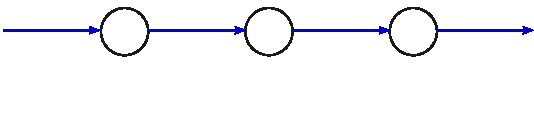
\includegraphics[width=\textwidth]{graphics/definition/mp-sequence.pdf}
    }%
    \only<2>{%
      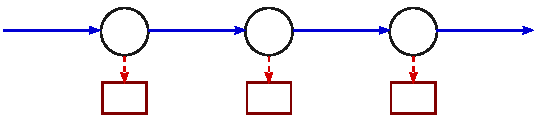
\includegraphics[width=\textwidth]{graphics/definition/hmm-sequence.pdf}
    }%
  }
\end{frame}


%%%%%%%%%%%%%%%%%%%%%%

%%%%%%%%%%%%%%%%%%%%%%
%% Slide 2: Construim un exemplu
\begin{frame}
  \frametitle{Exemplu: Urmărirea stărilor emoționale}
  \begin{columns}[T]
    \column{0.58\textwidth}
    \only<1>{\framebox{
\includegraphics[width=\textwidth]{graphics/toy-example/example-k.pdf}}}%
    \only<2>{\framebox{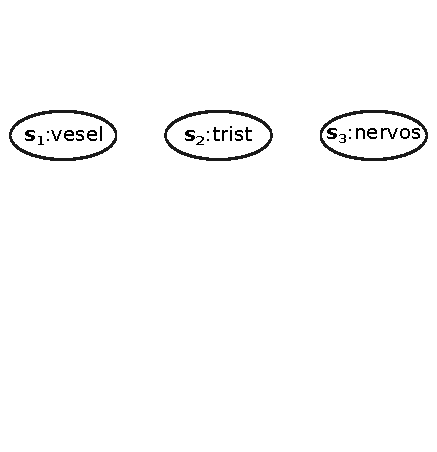
\includegraphics[width=\textwidth]{graphics/toy-example/example-l.pdf}}}%
    \only<3>{\framebox{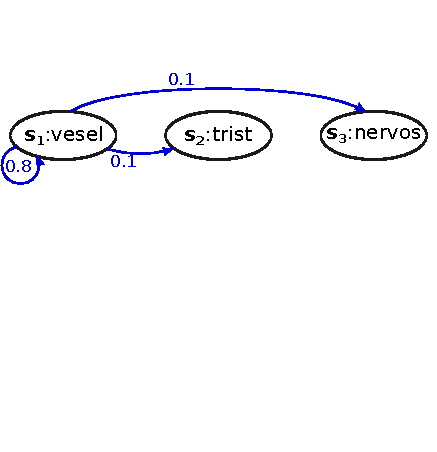
\includegraphics[width=\textwidth]{graphics/toy-example/example-m.pdf}}}%
    \only<4>{\framebox{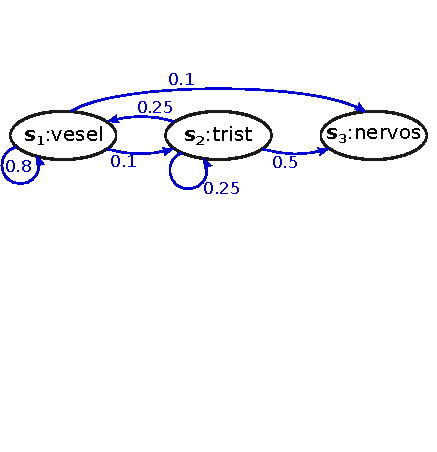
\includegraphics[width=\textwidth]{graphics/toy-example/example-n.pdf}}}%
    \only<5>{\framebox{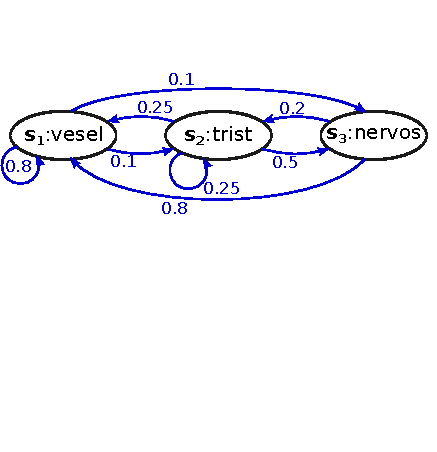
\includegraphics[width=\textwidth]{graphics/toy-example/example-o.pdf}}}%
    \only<6>{\framebox{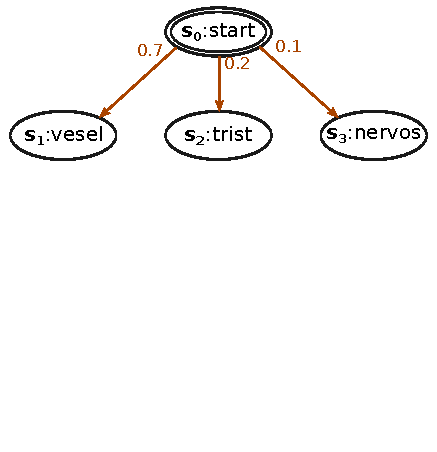
\includegraphics[width=\textwidth]{graphics/toy-example/example-p.pdf}}}%
    \only<7>{\framebox{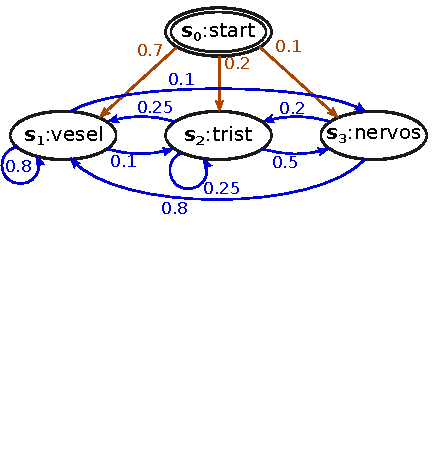
\includegraphics[width=\textwidth]{graphics/toy-example/example-q.pdf}}}%
    \only<8>{\framebox{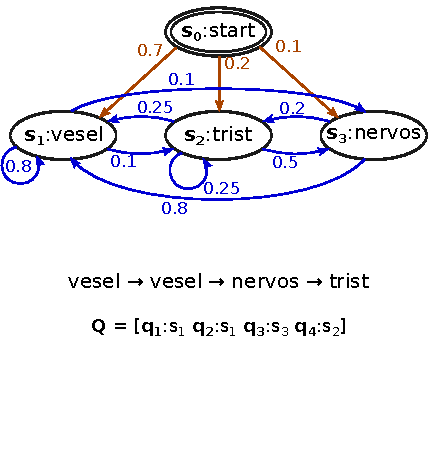
\includegraphics[width=\textwidth]{graphics/toy-example/example-r.pdf}}}%
    \only<9>{\framebox{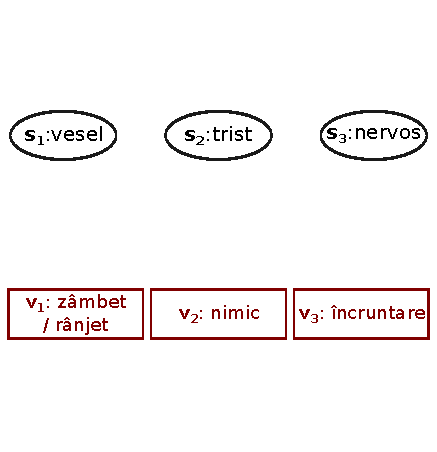
\includegraphics[width=\textwidth]{graphics/toy-example/example-s.pdf}}}%
    \only<10>{\framebox{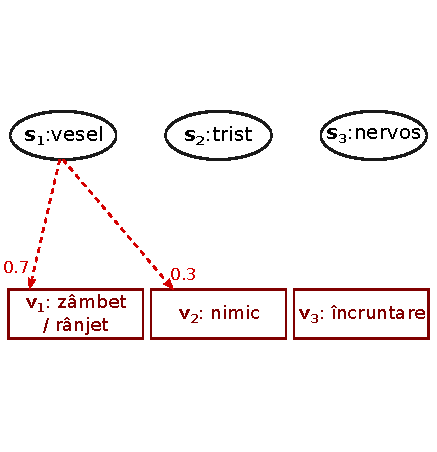
\includegraphics[width=\textwidth]{graphics/toy-example/example-t.pdf}}}%
    \only<11>{\framebox{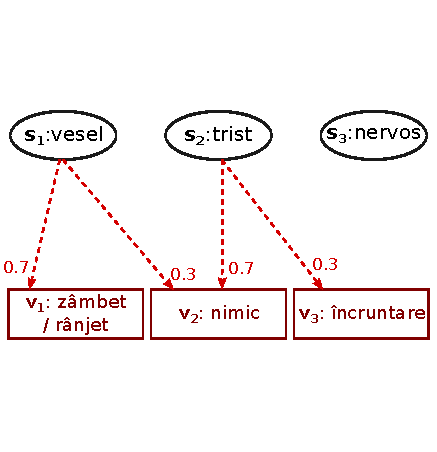
\includegraphics[width=\textwidth]{graphics/toy-example/example-t2.pdf}}}%
    \only<12>{\framebox{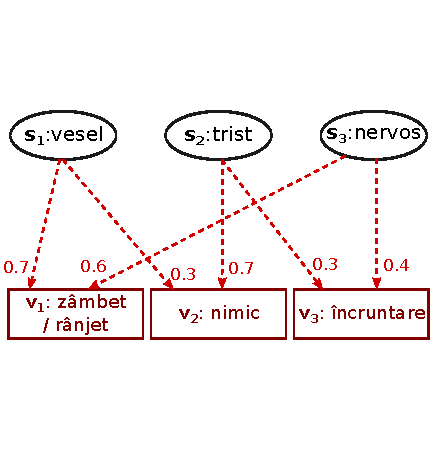
\includegraphics[width=\textwidth]{graphics/toy-example/example-u.pdf}}}%
    \only<13>{\framebox{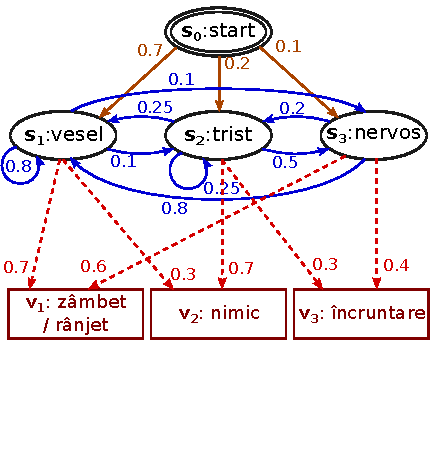
\includegraphics[width=\textwidth]{graphics/toy-example/example-v.pdf}}}%
    \only<14>{\framebox{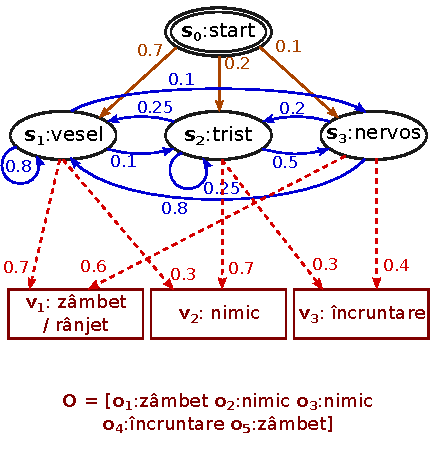
\includegraphics[width=\textwidth]{graphics/toy-example/example-w.pdf}}}%
    \only<15>{\framebox{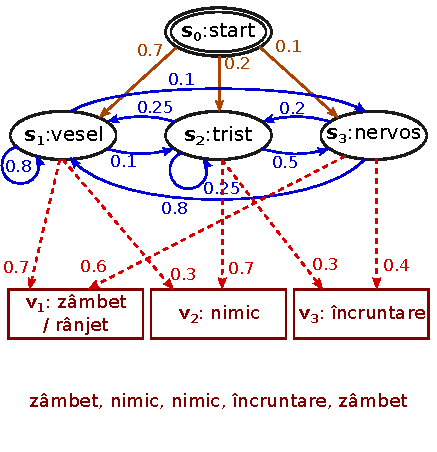
\includegraphics[width=\textwidth]{graphics/toy-example/example-x.pdf}}}%
    \only<16>{\framebox{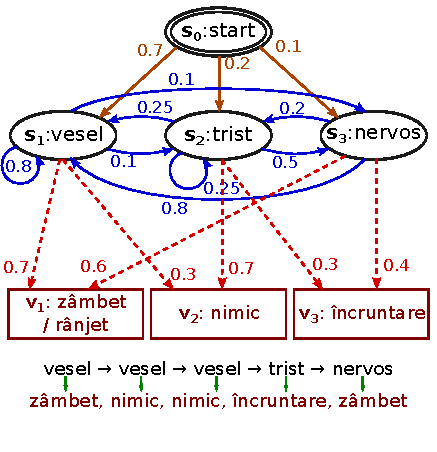
\includegraphics[width=\textwidth]{graphics/toy-example/example-y.pdf}}}%
    \only<17>{\framebox{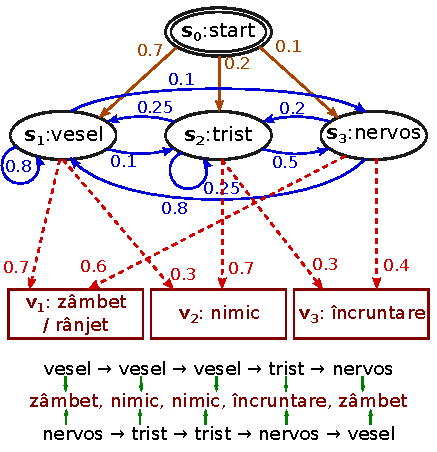
\includegraphics[width=\textwidth]{graphics/toy-example/example-z.pdf}}}%
    \column{0.4\textwidth}%
    \only<1>{%
      Să considerăm următorul exmeplu:
      \begin{itemize}
      \item un robot ce urmărește evoluția stărilor emoționale ale
        unui om
      \end{itemize}
      \vspace*{1em} Senzor:
      \begin{itemize}
      \item cameră video
      \end{itemize}
      \vspace*{1em}
      Exemplu adaptat după :\\\vspace*{.5em}
      \def\newblock{}\nobibliography{}\bibentry{zubek2006introduction}
    }\only<2>{%
      $\mathbf{N}$ - numărul de stări ascunse\\%
      $\mathbf{S}$ - mulțimea stărilor\\\vspace*{.5em}%
      \horiline%
      $\mathbf{N}=3$ \\\vspace*{.5em}%
      Stări:
      \begin{itemize}
      \item $\mathbf{s_1}$: vesel
      \item $\mathbf{s_2}$: trist
      \item $\mathbf{s_3}$: nervos
      \end{itemize}
    }\only<3-5>{%
      $\mathbf{A}$ - matricea distribuțiilor de
      probabilitate ale tranzițiilor între stări\\\vspace*{.5em}%
      \small{%
        $\mathbf{A} = \lbrace a_{i,j} \rbrace, \: 1 \le i, j \le N$\\\vspace*{.5em}%
        $a_{i,j} = P(q_{t+1}=s_j \vert q_t = s_i)$\\%
        \horiline%
        $\displaystyle\sum_{j=1}^{N}a_{i,j}=1, \quad 1 \le i \le N$}\\%
      \horiline%
      \visible<3->{%
        $\mathbf{A} = \bordermatrix{~ & s_1 &
          s_2 & s_3 \cr s_1 & 0.8 & 0.1 & 0.1 \cr s_2 &
          \visible<4->{0.25} & \visible<4->{0.25} & \visible<4->{0.5}
          \cr s_3 & \visible<5->{0.8} & \visible<5->{0.2} &
          \visible<5->{0} \cr}$ }%
    }\only<6>{%
      $\mathbf{\Pi}$ - distribuția stării inițiale\\\vspace*{0.5em}%
      $\mathbf{\Pi} = \lbrace \pi_i \rbrace,\quad 1 \le i \le N$\\\vspace*{0.5em}%
      $\pi_i = P(q_1 = s_i)$\\\vspace*{0.5em}%
      $\mathbf{\Pi} = \bordermatrix{ ~ & s_1 & s_2 & s_3 \cr ~ & 0.7 & 0.2 & 0.1 \cr}$%
    }\only<7-8>{%
      Deocamdată am descris un \emph{proces Markov}.\\\vspace*{0.25em}%
      $A = \bordermatrix{~ & s_1 & s_2 & s_3 \cr s_1 & 0.8 & 0.1 & 0.1 \cr s_2
        & 0.25 & 0.25 & 0.5 \cr s_3 & 0.8 & 0.2 & 0 \cr}$\\\vspace*{0.25em}%
      $\Pi = \bordermatrix{ ~ & s_1 & s_2 & s_3 \cr ~ & 0.7 & 0.2 & 0.1 \cr}$\\%
      \horiline%
      \visible<8>{%
        Notație: $\mathbf{Q} = [ q_1 q_2 \cdots q_T ]$%
        \horiline%
        \begin{equation*}
          \begin{array}{l}
            \scriptstyle
              P(Q \vert A,\Pi) = \pi_{q_1}a_{q_1,q_2}\cdots a_{q_{T-1},q_T} \\
              \scriptstyle
              P(s_1,s_1,s_3,s_2\vert A,\Pi) = \pi_1 \cdot a_{1,1} \cdot a_{1,3} \cdot a_{3,2}= \\
              \scriptstyle
              = 0.8\; \cdot\; 0.8\; \cdot\; 0.1\; \cdot\; 0.2 = 0.0128
          \end{array}%
        \end{equation*}%
      }}\only<9>{%
      $\mathbf{M}$ - numărul de valori observabile distincte\\\vspace*{.5em}%
      $\mathbf{M}=3$\\\vspace*{.5em}
      valori observabile:
      \begin{itemize}
      \item $\mathbf{v_1}$: zâmbmet / rânjet
      \item $\mathbf{v_2}$: nimic
      \item $\mathbf{v_3}$: încruntare
      \end{itemize}%
    }\only<10-12>{%
      $\mathbf{B}$ - matricea distribuțiilor de probabilitate ale valorilor
      observabile\\\vspace*{.5em}
      \small{% 
        $\mathbf{B} = \lbrace b_{j,k} \rbrace \: \scriptstyle{1
          \le j \le N, 1 \le k, \le M}$
        \begin{equation*}
          \begin{split}
            b_{j,k} & =b_{j}(v_k) \\
            & =P(o_t = v_k \vert q_t = s_j)
          \end{split}
        \end{equation*}%
        \vspace*{-.5em}\horiline%
        $\displaystyle\sum_{k=1}^{M}b_{j,k}=1, \quad 1 \le j \le N$%
      }%
      \horiline%
      \visible<10->{ $\mathbf{B} = \bordermatrix{~ & v_1 &
          v_2 & v_3 \cr s_1 & 0.7 & 0.3 & 0 \cr s_2 &
          \visible<11->{0} & \visible<11->{0.7} & \visible<11->{0.3}
          \cr s_3 & \visible<12->{0.6} & \visible<12->{0} &
          \visible<12->{0.4} \cr}$}%
    }\only<13>{% 
      $\mathbf{\lambda}$ - parametrii Modelului Markov Ascuns\\\vspace*{.5em}%
      $\lambda = (A, B, \Pi)$\\\vspace*{2em}%
      $A$ - matricea distribuțiilor de probabilitate ale tranzițiilor între
      stări\\\vspace*{.5em}%
      $B$ - matricea distribuțiilor de probabilitate ale valorilor observabile\\\vspace*{.5em}%
      $\Pi$ - distribuția stării inițiale%
    }\only<14-17>{%
      $\mathbf{O}$ - secvența de observații\\\vspace*{1em}%
      $\mathbf{T}$ - lungimea secvenței de observații\\\vspace*{1em}%
      $O = [ o_1 o_2 \cdots o_T ]$% 
    }%
  \end{columns}
\end{frame}
%%%%%%%%%%%%%%%%%%%%%%

%%%%%%%%%%%%%%%%%%%%%%
%% Slide 3: Din ce este compus un HMM
\begin{frame}
  \frametitle{Modele Markov Ascunse}
  \begin{block}{Definiție}
    Un \alert{Model Markov Ascuns} este un tuplu $\langle S,V,A,B,P \rangle$:
    \begin{itemize}
    \item $S$ - mulțimea stărilor
    \item $V$ - mulțimea valorilor observabile
    \item $A$ - matricea de tranziție
    \item $B$ - matricea de emisie
    \item $\Pi$ - matricea distribuției stării inițiale
    \end{itemize}
  \end{block}
  \begin{itemize}
  \item Notație: $\lambda=(A,B,\Pi)$ - parametrii modelului
  \end{itemize}
  \vspace*{.5em}
  \begin{center}%
    \framebox{%
      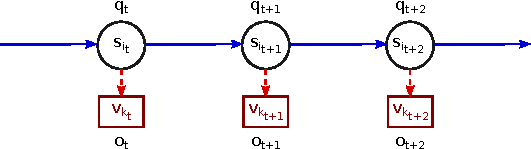
\includegraphics[width=.6\textwidth]{graphics/definition/hmm-sequence-adnotated.pdf}%
    }%
  \end{center}
\end{frame}
%%%%%%%%%%%%%%%%%%%%%% 


%%%%%%%%%%%%%%%%%%%%%%
%% Slide 4: Problema evaluării

\begin{frame}[T]
  \frametitle{Reformularea problemelor fundamentale ale MMA}
  \begin{block}{Problema evaluării}
    Date fiind un model \visible<2->{\alert{$\lambda=(A,B,\Pi)$}} și o
    secvență de observații \visible<2->{\alert{$O = [ o_1 o_2 \cdots
        o_T ]$}}, cum calculăm probabilitatea \visible<2->{\alert{$P(O
        \vert \lambda)$}} ca secvența de observații să fi fost
    generată de acel model?
  \end{block}
  \visible<3->{%
    \begin{itemize}
    \item Prin enumerarea tuturor secvențelor posibile de stări:
      \begin{equation}
          P(O \vert \lambda) = \displaystyle\sum_{\text{all}\;Q} P(O
          \vert Q, \lambda) \cdot P(Q \vert \lambda)
        \label{eq1}
      \end{equation}
      (legea probabilității totale)
    \end{itemize}
  }
\end{frame}

%%%%%%%%%%%%%%%%%%%%%%
%% Slide 5: Prelucrarea formulei

\begin{frame}[t]
  \frametitle{Reformularea problemelor fundamentale ale MMA}
  \vspace*{-1em}%
  \begin{equation}
      P(O \vert \lambda) = \displaystyle\sum_{\text{all}\;Q} P(O \vert
      Q, \lambda) \cdot P(Q \vert \lambda)
    \tag{\ref{eq1}}
  \end{equation}%
  \horiline%
  \visible<2->{%
    \small{Primul factor (independență condițională):}
    \begin{equation}
      P(O \vert Q, \lambda) = \displaystyle\prod_{t=1}^{T} P(o_t \vert
      q_t, \lambda)= \displaystyle\prod_{t=1}^{T} b_{q_t}(o_t) =
      b_{q_1}(o_1) \cdot \ldots \cdot b_{q_T}(o_T)
      \label{eq:pql}
    \end{equation}%
    \visible<3->{%
      \small{Al doilea factor (presupunerea Markov):}
      \begin{equation}
        P(Q | \lambda) = \pi_{q_1}\displaystyle\prod_{t=2}^{T}
        a_{q_{t-1},q_t} = \pi_{q_1} \cdot a_{q_1,q_2} \cdot a_{q_2,q_3} \cdot \ldots \cdot
        a_{q_{T-1},q_T}\label{eq:pql2}
      \end{equation}%
      \horiline%
      \visible<4->{%
        \begin{equation}
          P(O \vert \lambda)  = \displaystyle\sum_{\text{all}\;Q} \Big( \pi_{q_1} \cdot
            b_{q_1}(o_1) \cdot \displaystyle\prod_{t=2}^{T} b_{q_t}(o_t)
            a_{q_{t-1},q_t} \Big)
          \tag{\ref{eq1}}
        \end{equation}
      }%
    }%
  }%
\end{frame}
%%%%%%%%%%%%%%%%%%%%%%

%%%%%%%%%%%%%%%%%%%%%%
%% Slide 6: Problema 2
\begin{frame}
  \frametitle{Reformularea problemelor fundamentale ale MMA}
  \begin{block}{Problema interpretării unei secvențe de observații}
    Date fiind un model \visible<2->{\alert{$\lambda=(A,B,\Pi)$}} și o
    secvență de observații \visible<3->{\alert{$O = [ o_1 o_2 \cdots
        o_T ]$}}, cum alegem o secvență corespunzătoare de stări
    \visible<4->{\alert{$Q = [ q_1 q_2 \cdots q_T ]$}} care \emph{să
      dea un înțeles} observațiilor? Cum \emph{descoperim} partea
    ascunsă a modelului?
  \end{block}
  \visible<5->{%
    \begin{itemize}
    \item Există mai multe criterii pentru \emph{cea mai bună} sevență
      \begin{itemize}
      \item Secvența celor mai probabile stări (luate individual):
        \begin{equation}
          \label{eq:inidi}
          Q_{\text{best}} = [\hat{q}_1\; \hat{q}_2\; \ldots \hat{q}_T], 
          \quad \hat{q}_t = \underset{s_i}{argmax}\; P(q_t = s_i \vert O, \lambda)
        \end{equation}%
        \visible<6->{\item Cea mai bună $cale$ (de dimensiune $T$)
          \begin{equation}
            Q_{\text{best}} = \underset{Q}{\operatorname{argmax}}\;
            P(Q \vert O, \lambda)
            = \underset{Q}{\operatorname{argmax}}\; P(Q, O \vert \lambda)
            \label{eq:best-explanation}
          \end{equation}}
      \end{itemize}
    \end{itemize}
  }%
\end{frame}

%%%%%%%%%%%%%%%%%%%%%%
%% Slide 7: Problema 3

\begin{frame}
  \frametitle{Reformularea problemelor fundamentale ale MMA}
  \begin{block}{Problema Estimării Modelului (Învățării)}
    Date fiind niște secvențe de observații
    \visible<2->{\alert{$\mathcal{O} = [O_1 O_2 \cdots O_L]$}}, cum
    \emph{ajustăm} \alert{parametrii}
    \visible<3->{\alert{$\lambda=(A,B,\Pi)$}} ai unui MMA astfel încât
    să explice cel mai bine observațiile?
  \end{block}
  \visible<4->{
    \begin{itemize}
    \item Întrebarea se poate reformula matematic:
      \begin{equation}
        \lambda_{\text{best}} = \underset{\lambda}{\operatorname{argmax}}\;
        P(\mathcal{O} \vert \lambda)
        \label{eq:best-explanation}
      \end{equation}
    \end{itemize}
  }
\end{frame}
%%%%%%%%%%%%%%%%%%%%%%
